\documentclass[12pt]{article}
\usepackage{amsmath}
\usepackage{graphicx}
\usepackage{fancyhdr}
\usepackage{hyperref}
\usepackage{listings}
\usepackage{times}
\usepackage{booktabs}
\usepackage{placeins}
\usepackage{xcolor}  % Optional: for color syntax highlighting

% Page Setup
\usepackage[a4paper, margin=1in]{geometry}

% Font Settings
\renewcommand{\rmdefault}{ptm} % Times New Roman font

% Spacing
\linespread{1.0} % Single spacing

% Set up the header and footer
\pagestyle{fancy}
\fancyhf{}
\fancyhead[L]{6.419x Module 3}
\fancyhead[C]{Written Report}
\fancyhead[R]{Your Name}

% Title Section
\title{Written Report – 6.419x Module 3}
\author{Evan Woods}
\date{}

\begin{document}

\maketitle

% Table of Contents
\tableofcontents
\newpage


\noindent \textbf{Name:} Evan Woods \\
\noindent \textbf{Module:} 6.419x Module 3

\section{Part 1: Thesis}

\textit{Clearly states a sociological question which is interesting and relevant to the data. The question must be sociologically motivated: for example, “Compare the network structure in 2003 vs 2009" is not a good question, without further context. If you have some reason to believe that the network structure changes in those years, then you should make that your central question: for example, “Did crimes involving youth offenders become more organized and structured over the years" is a better question, from which comparing the structure in different years becomes part of the methodology to answer the question. More examples of possible questions for cooffending networks are provided below. }

Parkinson's is a disease that affects the social and cognitive abilities of people who have the diagnosis. In this body of work, I sought to identify which patients in a dataset are either cognitively normal, under mild cognitive impairment (hereafter refered to as MCI), or have Parkinson's disease dementia (hereafter refered to as PDD) based on computed fractional Amplitude Low-Frequency Fluctuations (hereafter refered to as fALFF) from the mean of the Blood Oxidation Level Dependent (hereafter refered to as BOLD) signal of the Substantia Nigra extracted from their functional Magnetic Resonance Image (hereafter refered to as fMRI). I furthered this analysis by seeking to answer the question: of the patients who have been identified to belong to the same diagnosis, what regions of the brain have no statistically significant difference of correlations of fALFF values? That is to say, what regions of the brain are similar in BOLD activity in patients with a common diagnosis, how does the activity of these patients differ between the diagnosed groups, and what are possible remedies to induce healthy levels of cognition determined by the fALFF of the BOLD signal in patients diagnosed with MCI or PDD to achieve an fALFF of the BOLD signal that resembles that of the patients diagnosed to be cognitively normal?   

\section{Part 2: Methods}

\textit{ (2 points) Describes methodology for network analysis.}
\textit{(2 points) Grader is convinced that the methodology makes sense for the question to be answered. Grader is convinced that no additional methodology within the bounds of techniques taught and discussed in this module could be applied beyond what was described. The grader should only consider additional methodology that adds meaningfully to the answer for the question: additions that simply repeat or confirm the presented results should not be considered by the grader. If a justification is provided for why a particular method was not used, the grader should be convinced by that argument. }

The data was collected as an OpenNeuro dataset on \href{https://openneuro.org/datasets/ds004392/versions/1.0.0}{Parkinson's Disease, functional connectivity, and cognition} \cite{ds004392:1.0.0}. In the dataset, all patients were diagnosed with Parkinson's, scanned with resting state fMRI, and underwent a neurocognitive test battery. Of these patients, there are three sub-diagnoses of patients who are either cognitively normal, have mild cognitive impairment, or have Parkinson's disease dementia. The patients were given scores of their attention, executive function, global cognition, language cognition, and visuospatial cognition based as determined by the results of the neurocognitive test battery. The eleven tests included a total score on the Montreal Cognitive Assessment, a Mattis Dementia Rating Scale 2, a Trail Making Test part A, a Trail Making Test part B, a Brief Test of Attention, an oral Symbol Digits Modality Test, a Boston Naming Test, a California Verbal Learning Test (2nd edition with the total learning score calculated from the 5 total trials), another California Verbal Learning Test (2nd edition with a long delay free recall total score), a F-A-S Verbal Phonemic Fluency test, and a Judgement of Line Orientation test. All units of the metrics which resulted from the tests were standardized with a norm of 0 and a variance of 1.

fALFF values have been indicative of cognitive function. A study titled "Default mode network mediates low‐frequency fluctuations in brain activity and behavior during sustained attention" indicates that "...low‐frequency fluctuations were significantly increased in the (Default Mode Network) but not in the (Anterior Nucleus) during sustained attention..." \cite{35903957}. This information was leveraged to assert fALFF as a key indicator metric of cognitive ability in the data. Furthermore, failure of the mitochondria to process reactive oxygen species in neuronal cells causes dopaminergic oxidation to cause cell damage, increased brain acidity, and cell death \cite{https://doi.org/10.1111/acel.13031}. This oxidative stress has been observed with respect to cell aging in the substantia nigra and is a cause of Parkinson's disease.

To calculate the fALFF scores of the BOLD signal from the fMRI data, the BOLD signal would need to first be derived from the fMRI data, and the fALFF calculated from this signal per patient per region. Once the fALFF scores were gathered and missing data imputed given the best hyperparameter of 2 k-nearest-neighbors, spectral clustering of the scaled fALFF of the Substantia Nigra region implementing 3 K-Means clusters with a nearest neighbors affinity as hyperparameters would create label predictions of the data. The integrity of the predicted clusters was verified by calculating the silhouette score of the labels and scaled data as well as calculating the convex Hull Ratio as the proportion of the hull volume of the scaled fALFF score of the substantia nigra per the data volume of the product of the peak-to-peak values of the scaled fALFF of the substantia nigra. The scaled fALFF scores of the substantia nigra were reduced to the first two principal components with principal component analysis (hereafter refered to as PCA), before a non-linear T-Stochastic Neighbor Embedding (hereafter refered to as T-SNE) further transformed the data so clear clusters would be identified on a plot. These cluster labels where then presumed as ground truth diagnoses for the patients. 

Using these clusters, the distribution of the results of the neurocognitive test battery and scores were graphed and inspected. A heatmap of the correlations of the scaled fALFF of the substantia nigra with respect to the cluster assignments, the left and right substantia nigra fALFF, and the as well as the F-A-S Verbal Phonemic Fluency test was visually inspected to determine which metric was indicative of cluster assignment. 

The patients fALFF scores for each region were then grouped by cluster and correlations with respect to the right substantia nigra were visually inspected. To determine which correlated regions had no statistically significant difference in correlation to the fALFF of the right substantia nigra of the patients in a common cluster, a z-test was implemented by calculating a z-score using the standard deviation of the correlations to the fALFF of the substantia nigra per the difference in the correlated fALFF scores. The critical value was calculated with a presumed normal probability distribution and significance level of 0.05. Regions that had no statistical significant difference in correlation to the fALFF of the right substantia nigra became nodes of a common network. The edges between the identified regions and the right substantia nigra were weighted by the correlations in the fALFF scores of the right substantia nigra. This method was followed for each of the three groups: cognitively normal, MCI, and PDD. The resulting graphs where then color-coordinated to delinate differences between clustered groups and combined into a single network graph. Three dimensional coordinates of the centroids from the anatomical NIFTI images in the dataset used to identify parcellated voxels of the brain regions were calculated and used to plot the nodes on a near-anatomically-correct 3-Dimensional model of the human brain collected from NIH \cite{NIH3DPX021161} and displayed on the \href{https://github.com/efwoods/Parkinson_Disease_Study}{GitHub - Parkinson's Disease Study} repository page: \href{https://efwoods.github.io/Parkinsons_Disease_Study/}{Parkinson's Disease Study} \cite{WoodsParkinsonsStudy}.

\section{Part 3: Results}
\textit{(2 points) Presents results, including figures and/or statistics, which address the question of interest.}
\textit{(2 points) The described methodology has been applied in complete and the results shown (that is, the author did not forget to include anything they discussed in the methodology.) }

The anatomical images were loaded from the dataset. An example of the anatomical image is shown in Figure \ref{fig:anatomy}.

\begin{figure}[h]  % "htbp" means "here, top, bottom, page" – LaTeX decides the best position
    \centering
    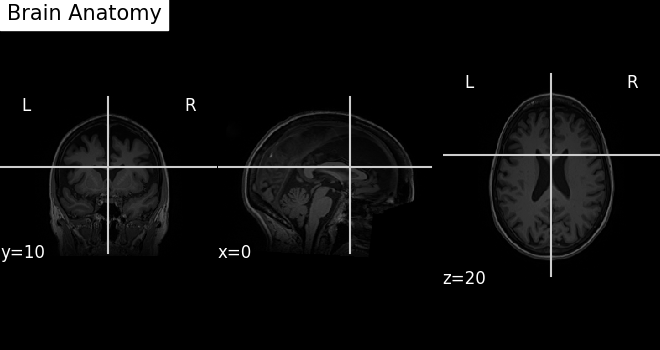
\includegraphics[width=\textwidth]{"../img/anatomy.png"}  % Replace with your image file name and path
    \caption{Example of the Anatomical Images of the Patients in the Dataset.}
    \label{fig:anatomy}  % Label for referencing the figure
\end{figure}

\FloatBarrier  % Forces all previous floats (tables, figures) to be processed.

Harvard-Oxford atlases where then used to segment and filter the fMRI data as shown in the regions of the cortex (shown in Figure \ref{fig:cortex}), subcortex (shown in Figure \ref{fig:subcortex}), and substantia nigra (as shown in Figure \ref{fig:SNR}). 

\begin{figure}[h]  % "htbp" means "here, top, bottom, page" – LaTeX decides the best position
    \centering
    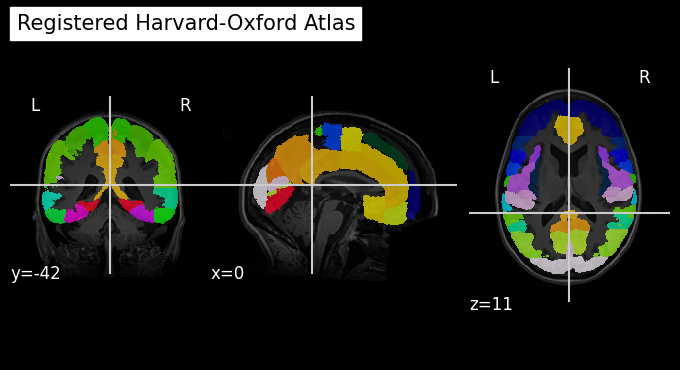
\includegraphics[width=\textwidth]{"../img/cortex.png"}  % Replace with your image file name and path
    \caption{Harvard-Oxford Atlas of the Cortical Regions of the Brain.}
    \label{fig:cortex}  % Label for referencing the figure
\end{figure}

\FloatBarrier  % Forces all previous floats (tables, figures) to be processed.

\begin{figure}[h]  % "htbp" means "here, top, bottom, page" – LaTeX decides the best position
    \centering
    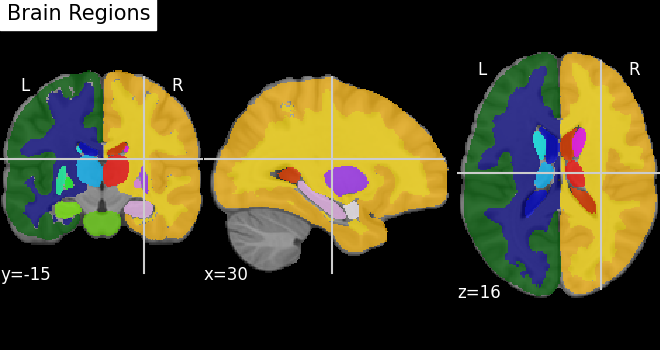
\includegraphics[width=\textwidth]{"../img/regions.png"}  % Replace with your image file name and path
    \caption{Harvard-Oxford Atlas of the Subcortical Regions of the Brain.}
    \label{fig:subcortex}  % Label for referencing the figure
\end{figure}

\FloatBarrier  % Forces all previous floats (tables, figures) to be processed.

\begin{figure}[h]  % "htbp" means "here, top, bottom, page" – LaTeX decides the best position
    \centering
    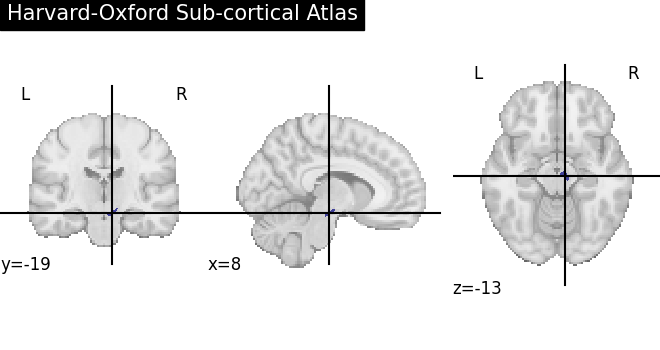
\includegraphics[width=\textwidth]{"../img/brain_atlas.png"}  % Replace with your image file name and path
    \caption{Atlas of the Right Substantia Nigra.}
    \label{fig:SNR}  % Label for referencing the figure
\end{figure}

\FloatBarrier  % Forces all previous floats (tables, figures) to be processed.

The the atlas served as a mask for the fMRI data to filter with respect to the region of interest. Then, the mean of the voxels of each brain region was calculated to create resulting BOLD signals. An example time series of a BOLD signal is shown in Figure \ref{fig:BOLD}.

\begin{figure}[h]  % "htbp" means "here, top, bottom, page" – LaTeX decides the best position
    \centering
    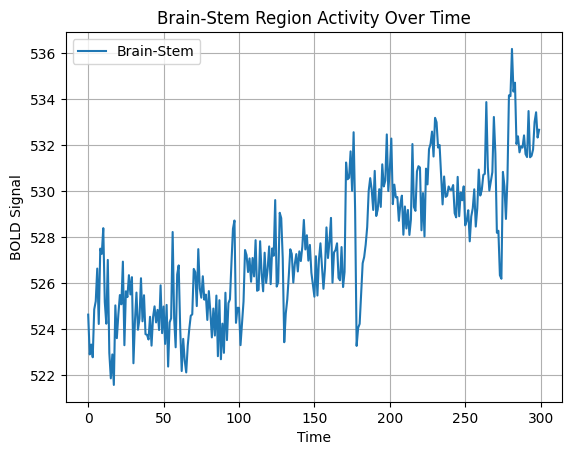
\includegraphics[width=\textwidth]{"../img/BOLD.png"}  % Replace with your image file name and path
    \caption{BOLD signal of the Brain Stem of a MCI Patient.}
    \label{fig:BOLD}  % Label for referencing the figure
\end{figure}

\FloatBarrier  % Forces all previous floats (tables, figures) to be processed.

To compute the fALFF, a low-frequency band of 0.01 to 0.1 Hz was established to detect Amplitude Low-Frequency Fluctuations (hereto refered to as ALFF). The fMRI data was sampled at 0.5 Hz or a sample every 2 seconds. The TR parameter was set to establish this information. A low-frequency mask was used along with a fast-fourier transform of the BOLD signal to inspect the frequency domain of each time series to identify the absolute value of the masked data. The total power among frequencies up to 0.25 were used to normalize this signal as to account for BOLD signal activity interactions across regions. The fALFF was computed as the proportion of the ALFF to the total power of the given BOLD signal. This computation is shown in Listing \ref{lst:fALFF_code}.

\begin{center}
    \begin{lstlisting}[caption={fALFF Calculation}, label={lst:fALFF_code}]
# Parameters
TR = 2 # Repetition time (in seconds)
low_freq_band = (0.01, 0.1) # Low-frequency range for ALFF (Hz)
n_timepoints = roi_df.shape[0]
frequencies = fftfreq(n_timepoints, d=TR)
fft_data = fft(roi_df.iloc[:, index], axis=-1)

# Create a mask for the low-frequency band
low_freq_mask = np.logical_and(
    frequencies >= low_freq_band[0], 
    frequencies <= low_freq_band[1])

# Compute the ALFF: average amplitude in the low-frequency band
alff = np.abs(fft_data)[..., low_freq_mask].mean(axis=-1)

# For fALFF: Compute the total power in the 0.01-0.25 Hz range
total_power = np.abs(fft_data)[..., 
    (frequencies >= 0.01) 
    & (frequencies <= 0.25)].sum(axis=-1)

# Compute fALFF: Normalized ALFF
falff = alff / total_power
\end{lstlisting}
\end{center}

\FloatBarrier

These fALFF values are expected to be in the range from 0 to 1 where 1 is indicative of high fluctuations of the BOLD signal,
and 0 is indicative of low fluctuations of the BOLD signal. The data was then scaled from -1 to 1 to normalize the data and process for clustering. To identify the appropriate clustering technique, the convexity of the data was investigated by calculating the Convex Hull Ratio as shown in Listing \ref{lst:convex_hull_code}.

\begin{center}
    \begin{lstlisting}[caption={Convex Hull Ration Calculation}, label={lst:convex_hull_code}]
hull = ConvexHull(fALFF_SN_scaled)

# Compute convex hull volume (or area in 2D)
hull_volume = hull.volume if fALFF_SN_scaled.shape[1] > 2 else hull.area

# Compute bounding box volume (approximation of occupied space)
# Range product as bounding box volume
data_volume = np.prod(np.ptp(fALFF_SN_scaled, axis=0))

# Convexity Ratio
convexity_ratio = hull_volume / data_volume
\end{lstlisting}
\texttt{Convexity Ratio: 0.3037}
\end{center}

A Convex Hull Ratio compares the volume (or area in 2D) of the convex hull enclosing the data to the actual volume occupied by the data points. The convexity ratio of the data is less than 1. In the Convex Hull Ratio, calculations close to 1 are convex as the "hull" is close to the data, and calculations much less than 1 are non-convex as the "hull" is further from the data resulting in a space between the hull and data. PCA works well to cluster convex data and will result in clusters that appear spherical in nature. In contrast, spectral clustering techniques are useful to cluster non-convex data that appears non-spherical under PCA projections. The middling values of the convexity ratio and the silhouette score indicate a good fit to the scaled fALFF data. The resulting clusters along with calculated means of each cluster group are shown in Figure \ref{fig:clustering}.

\FloatBarrier

\begin{figure}[h]  % "htbp" means "here, top, bottom, page" – LaTeX decides the best position
    \centering
    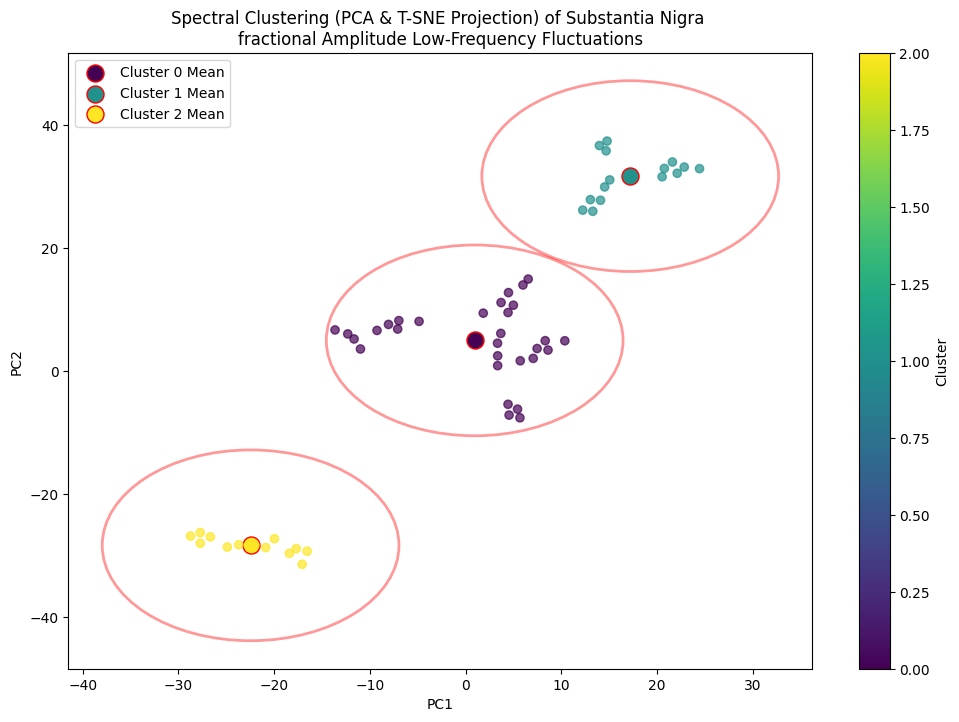
\includegraphics[width=\textwidth]{"../img/fALFF_SN_Spectral_Clustering.png"}  % Replace with your image file name and path
    \caption{Spectral Clustering of PCA and T-SNE Projection of the Right Substantia Nigra fALFF.}
    \label{fig:clustering}  % Label for referencing the figure
\end{figure}

\begin{center}
    \texttt{Silhouette Score: 0.3722}
\end{center}


\FloatBarrier  % Forces all previous floats (tables, figures) to be processed.

The means of each cluster is listed in Table \ref{tab:example}. In both substantia nigra left and substantia nigra right, the values are sequential from least to greatest. Presumably, the fALFF with diminished activity is the most intense diagnosis with cognitive normality at the opposite end of the spectrum as inferred from the research article \href{https://pmc.ncbi.nlm.nih.gov/articles/PMC9704793/}{Default mode network mediates low‐frequency fluctuations in brain activity and behavior during sustained attention} \cite{35903957}. Parkinson's Disease is not necessarily progressive toward these worsening impairments and patients may never experience any necessitated declination of health toward other clustered disorders. The dataset explicitly states that these three clusters exist \cite{ds004392:1.0.0}, and the visual plot as well as the silhouette and convex hull ratio calculations support this claim.

\begin{table}[ht]
\centering
\begin{tabular}{lrrl}
    \toprule
     & Substantia Nigra Left & Substantia Nigra Right & Cognitive Health \\
    Cluster &  &  &  \\
    \midrule
    0 & 0.332347 & -0.091915 & MCI \\
    1 & -1.161762 & -1.059544 & PDD \\
    2 & 0.573540 & 1.434661 & Cognitively Normal \\
    \bottomrule
\end{tabular}
\caption{Identification of Cognitive Health Based on Scaled PCA and T-SNE Projections of Spectrally Clustered fALFF metrics for the Right and Left Substantia Nigra.}
\label{tab:example}  % Label the table for referencing
\end{table}

\FloatBarrier  % Forces all previous floats (tables, figures) to be processed.

Given these defined clusters, further inquiry into the result of the neurocognitive battery of tests was made to determine if any separation with respect to the mean of the distribution of the data could be visually identified. Only the FAS Verbal Phonemic Fluency Test scores showed any discrepancy in the means between clustered groups as shown in Figure \ref{fig:pdf}.

\begin{figure}[h]  % "htbp" means "here, top, bottom, page" – LaTeX decides the best position
    \centering
    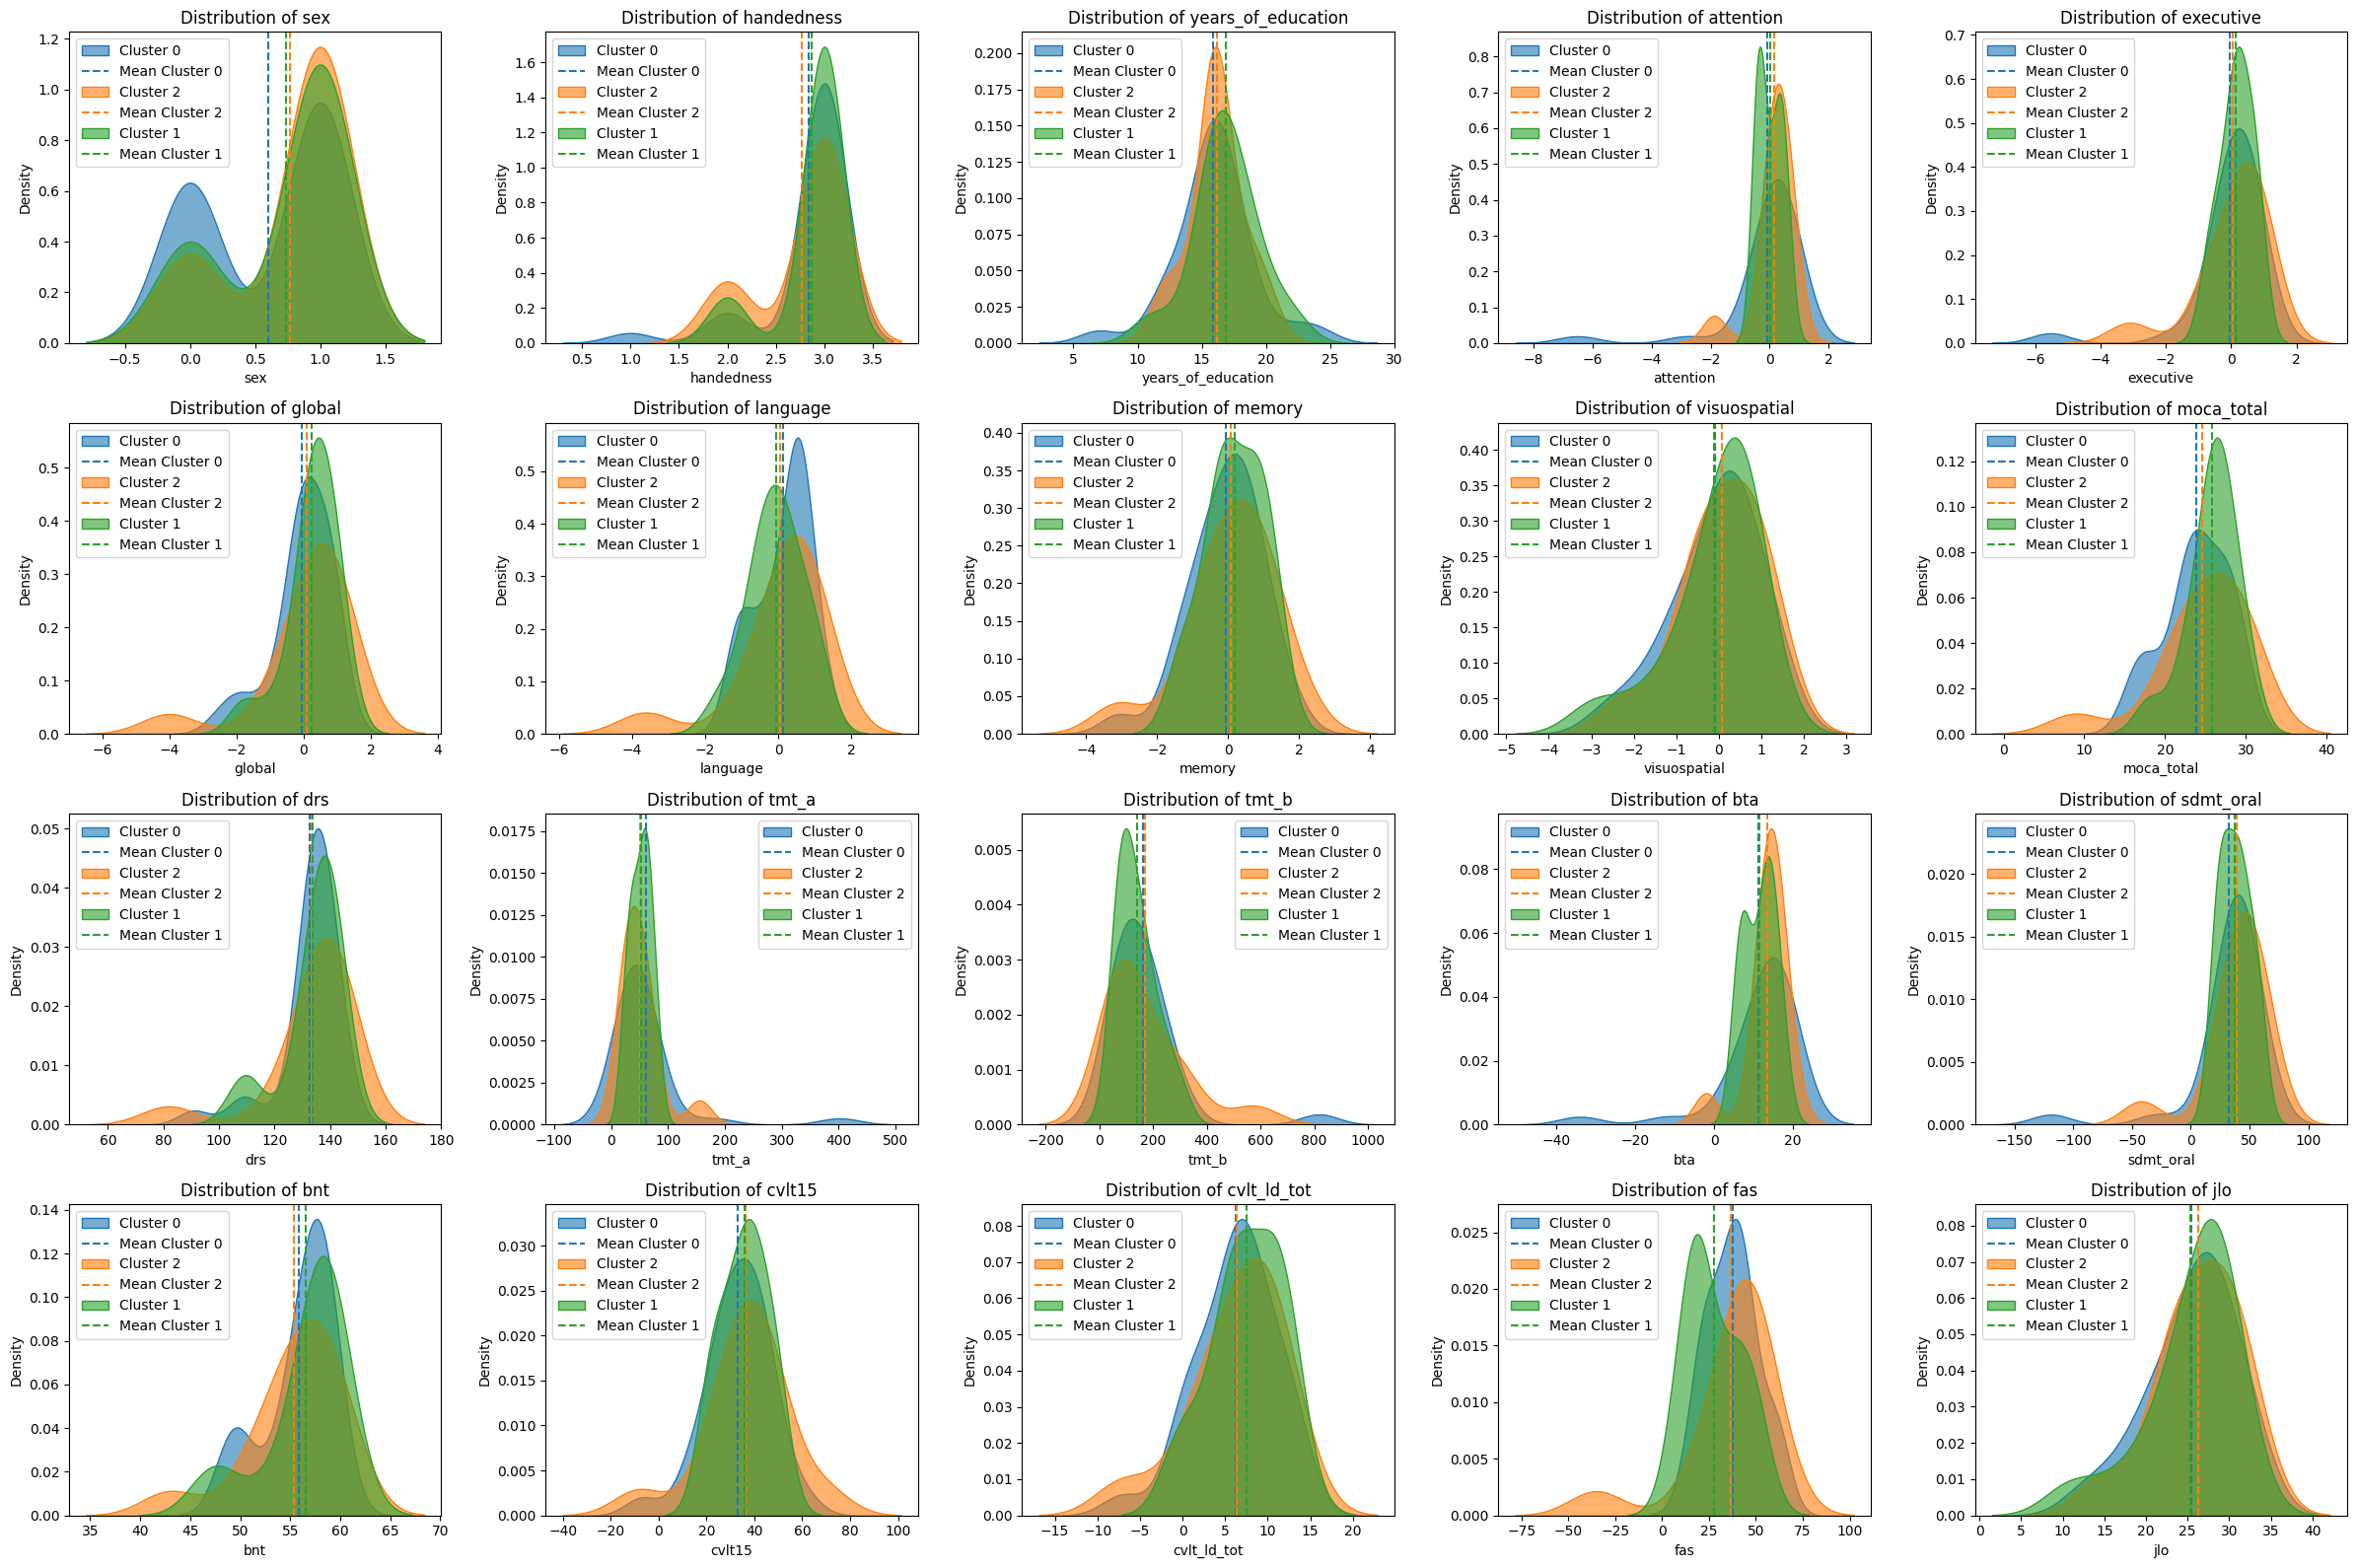
\includegraphics[width=\textwidth]{"../img/pdf_of_clustered_test_results.png"}  % Replace with your image file name and path
    \caption{Distribution of Neurocognitive Battery Test Results and Metrics Grouped by Cognitive Diagnosis.}
    \label{fig:pdf}  % Label for referencing the figure
\end{figure}

\FloatBarrier

A heatmap to determine the best indicator of cluster grouping given correlation with cluster assignment was generated as shown in Figure \ref{fig:heatmap}. The right substantia nigra proved to be most correlated to the cluster assignment and was therefore the basis of the network graph.

\begin{figure}[h]  % "htbp" means "here, top, bottom, page" – LaTeX decides the best position
    \centering
    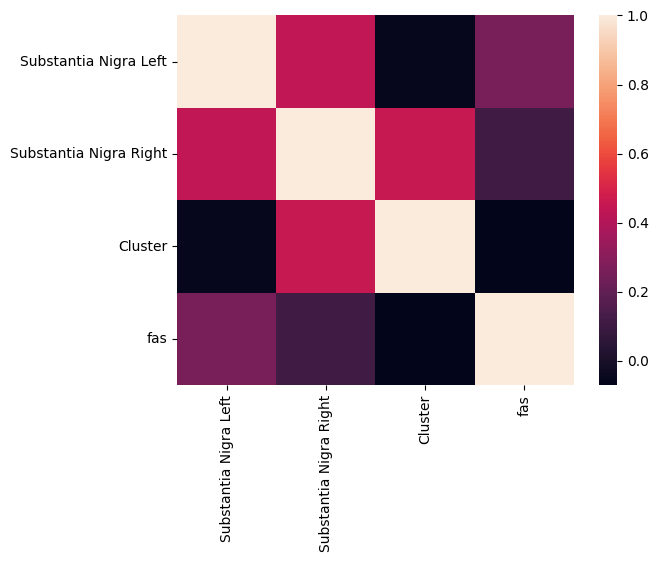
\includegraphics[width=\textwidth]{"../img/fALFF_SN_fas_test_correlation_heatmap.png"}  % Replace with your image file name and path
    \caption{This is the heatmap of correlations with respect to the substantia nigra left, the substantia nigra right, the cluster assignments, and the FAS Verbal Phonemic Fluency Test scores.}
    \label{fig:heatmap}  % Label for referencing the figure
\end{figure}

\FloatBarrier

Correlations of the fALFF scores with the right substantia nigra in each clustered group were computed. Brain regions whose fALFF correlations were not statistically significanly different from the right substantia nigra were added to each plot with the respective correlations shown on the y-axis and the region along the x-axis. This was computed to show how many regions had similar activity if the right substantia nigra was indicative of cognitive health per cluster assignment. Cognitively Normal Correlations are shown in Figure \ref{fig:cn}. No region was correlated within the MCI group as shown in Figure \ref{fig:mci}. Figure \ref{fig:pdd} shows that the left claudate had no statistical significant difference from the fALFF correlation of the right substantia nigra.

\begin{figure}[h]  % "htbp" means "here, top, bottom, page" – LaTeX decides the best position
    \centering
    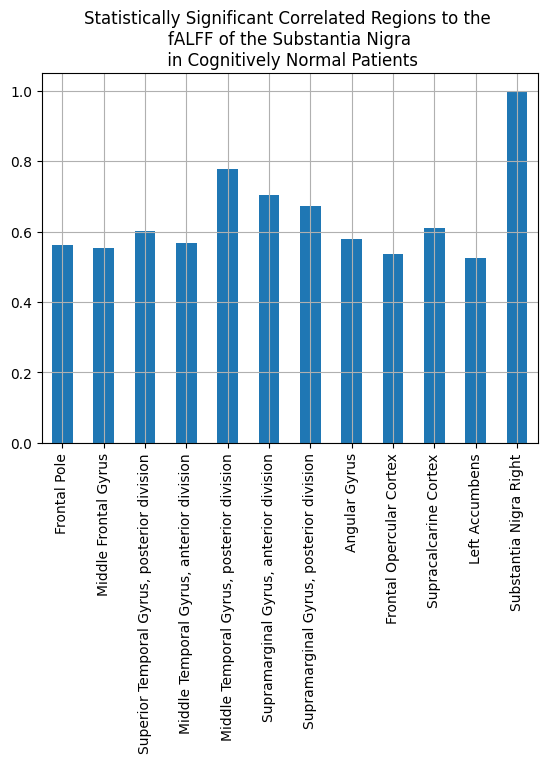
\includegraphics[width=\textwidth]{"../img/statistically_significant_correlated_regions_sn_cogn.png"}  % Replace with your image file name and path
    \caption{Bar Plot of Brain Regions with No Statistical Significant Difference in Correlation of fALFF with Respect to the Right Substantia Nigra fALFF among Cognitively Normal Parkinson's Disease Patients.}
    \label{fig:cn}  % Label for referencing the figure
\end{figure}

\FloatBarrier

\begin{figure}[h]  % "htbp" means "here, top, bottom, page" – LaTeX decides the best position
    \centering
    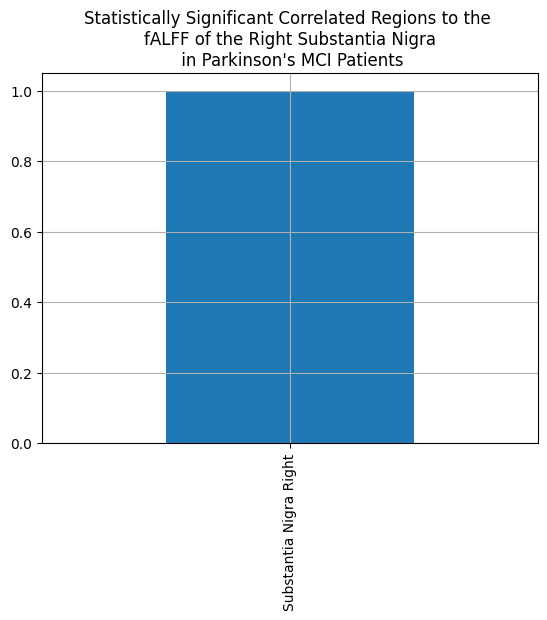
\includegraphics[width=\textwidth]{"../img/statistically_significant_correlated_regions_sn_mci.png"}  % Replace with your image file name and path
    \caption{Bar Plot of Brain Regions with No Statistical Significant Difference in Correlation of fALFF with Respect to the Right Substantia Nigra fALFF among Mild Cognitive Impaired Parkinson's Disease Patients.}
    \label{fig:mci}  % Label for referencing the figure
\end{figure}

\FloatBarrier


\begin{figure}[h]  % "htbp" means "here, top, bottom, page" – LaTeX decides the best position
    \centering
    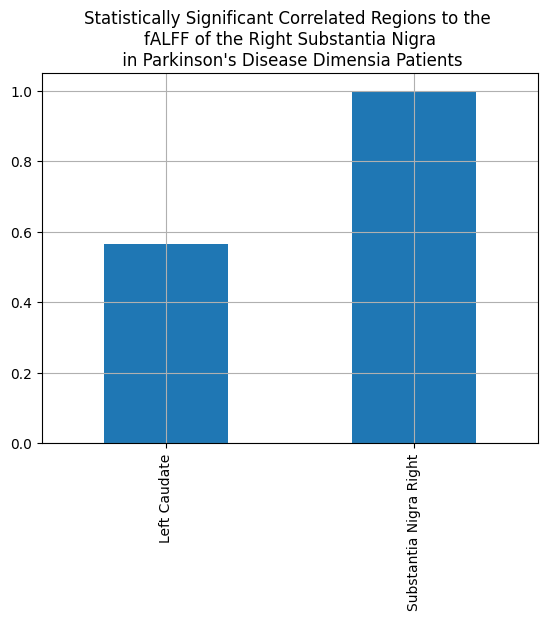
\includegraphics[width=\textwidth]{"../img/statistically_significant_correlated_regions_sn_pdd.png"}  % Replace with your image file name and path
    \caption{Bar Plot of Brain Regions with No Statistical Significant Difference in Correlation of fALFF with Respect to the Right Substantia Nigra fALFF among Parkinson's Disease Dementia Patients.}
    \label{fig:pdd}  % Label for referencing the figure
\end{figure}

\FloatBarrier

The undirected weighted network graph, shown in Figure \ref{fig:2D}, was defined where the nodes are the regions of the brain that had no statisticaly significant difference in correlation with the fALFF of the right substantia nigra for each group. The nodes were color-coded according to cluster assignment where green nodes indicate cognitively normal patients and red nodes indicate patients with PDD. The line thickness and shade are both scaled by the weight of the edges in the undirected network graph, and the central node is the substantia nigra as all correlations are with respect to this region which is indicative of cluster assignment as shown in the heatmap in Figure \ref{fig:heatmap}.

\begin{figure}[h]  % "htbp" means "here, top, bottom, page" – LaTeX decides the best position
    \centering
    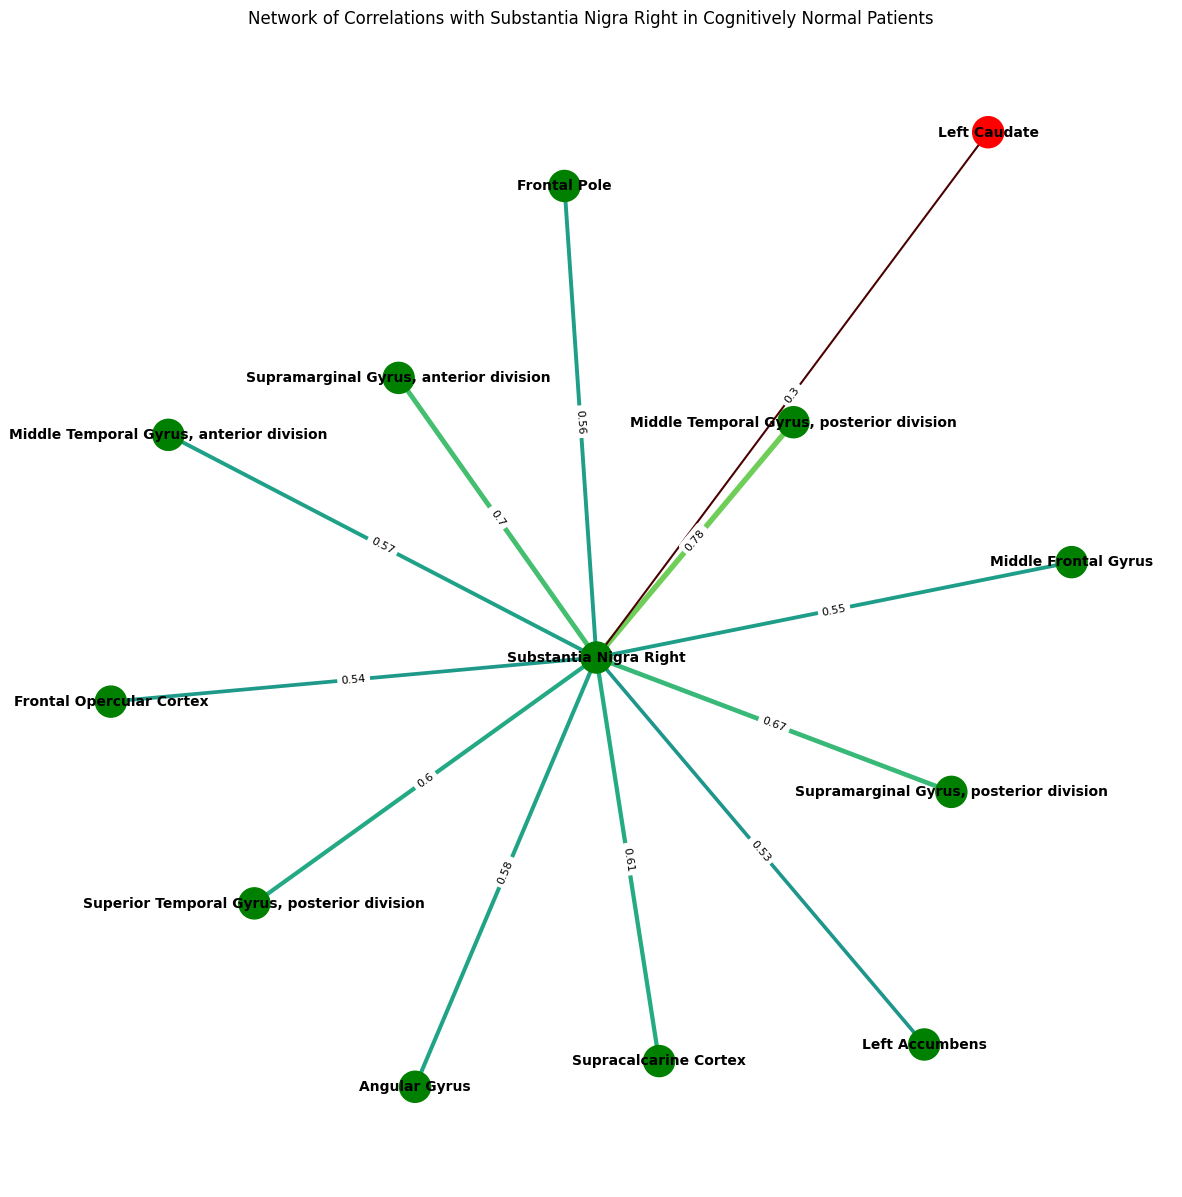
\includegraphics[width=\textwidth]{"../img/statistically_significant_correlated_regions_sn_cogn_pdd_graph.png"}  % Replace with your image file name and path
    \caption{2-Dimensional Undirected Weighted Network Graph of Brain Regions with Correlations with No Statistical Significant Difference of fALFF to the Right Substantia Nigra fALFF.}
    \label{fig:2D}  % Label for referencing the figure
\end{figure}

\FloatBarrier

A \href{https://3d.nih.gov/entries/3DPX-021161}{Detailed Human Brain Model (3D)} was acquire from the NIH website \cite{NIH3DPX021161}. This was used along with centroids that were calculated (along with the mean voxels that defined the BOLD signals) given regions of interest defined by the harvard-oxford atlases that masked the anatomical images from the dataset of the patients. These anatomically correct coordinates served as a guide to map the network graph into a 3-dimensional space to view relationships between regions of the brain common to a given diagnosis. This is shown in Figure \ref{fig:3D}. An interactive demonstration is available at the \href{https://efwoods.github.io/Parkinsons_Disease_Study/}{Parkinson's Disease Study repository Github Page} \cite{WoodsParkinsonsStudy}.

\begin{figure}[h]  % "htbp" means "here, top, bottom, page" – LaTeX decides the best position
    \centering
    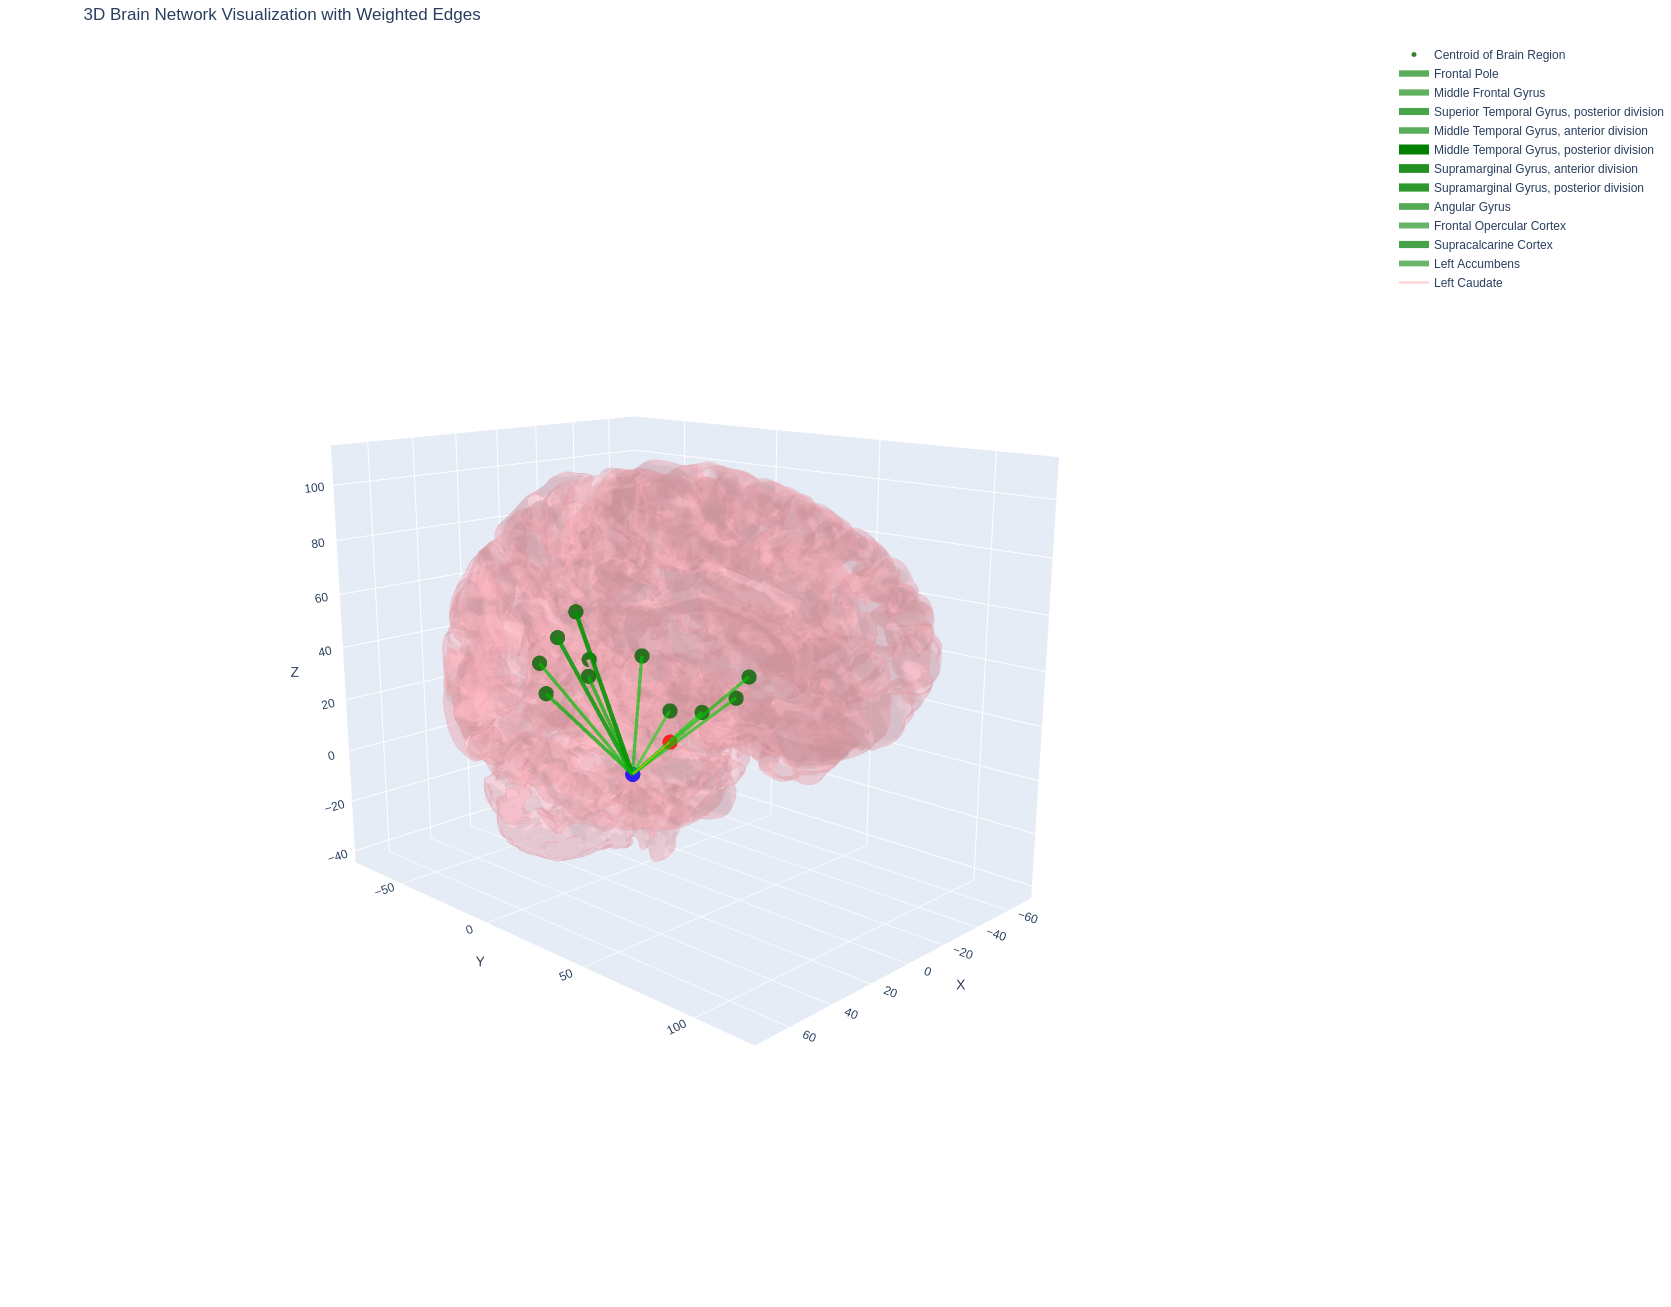
\includegraphics[width=\textwidth]{"../img/3D_Plot_of_Correlated_fALFF.png"}  % Replace with your image file name and path
    \caption{3-Dimensional Undirected Weighted Network Graph of Brain Regions with Correlations with No Statistical Significant Difference of fALFF to the Right Substantia Nigra fALFF.}
    \label{fig:3D}  % Label for referencing the figure
\end{figure}

\FloatBarrier

\section{Part 4: Discussion}
\textit{(2 points) Question does not need to be successfully answered, but the grader should be convinced that the author has answered the question to the best ability of the methodology presented.}
\textit{(1 point) Provides commentary on what was discovered, what were the limitations of the methods, what may have been surprising to discover, etc.}
\textit{(1 point) Award this point if the question was successfully answered to the grader's satisfaction. }

Figure \ref{fig:2D} shows that there are more brain regions with activity to the substantia nigra in cognitively normal patients. This is to be expected as other regions of the brain would have healthy BOLD signals as well as the substantia nigra region. 

The MCI group, shown in Figure \ref{fig:mci}, had no region that had no stastically significant difference from the substantia nigra fALFF. This indicates that the substantia nigra is not functioning like the BOLD signals of other regions of the brain for this group of diagnosed patients. This is to be expected when the substantia nigra is showing poor functional activity in the BOLD signal. 

The PDD group, shown in Figure \ref{fig:pdd}, showed correlation only with the left claudate which in located in the basal ganglia and is responsible for motor-coordinated tasks. This correlated fALFF values of BOLD signal activity with a low-active fALFF in the substantia nigra is indicative of Parkinson's that has affected both regions of the brain. 

Visualizations such as these are useful in depicting Parkinson's as a disease. The more that is known about the disease, the more readily abled doctor's are to combat it. With a condition such as this, awareness and prevention serve as best ailments, and visualizing activity of these regions as well as possibly predicting future BOLD signal declination are good measures of preventing poor cognitive health through proactive awareness for those that may be genetically or otherwise inclined to the disease. 


% Insert References Section
\bibliographystyle{plain} % Citation style (alternatives: abbrv, unsrt, apalike, IEEEtran, etc.)
\bibliography{references} % Use the .bib file (without the .bib extension)

\end{document}
